% =============================================================================
\section{Squeezing near a Feshbach resonance}
% =============================================================================

This section contains squeezing results from \cite{Opanchuk2012}.

\copypaste{copypaste begins}

\begin{figure}
    \centerline{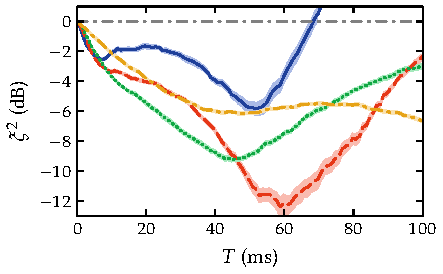
\includegraphics{figures_generated/bec_squeezing/feshbach_squeezing.pdf}}

    \caption{
    Wigner simulations of squeezing in the vicinity of $9.1\un{G}$ Feshbach resonance in \Rb.
    \todo{simulation parameters}.
    except for the inter-component scattering length and corresponding loss rate~\cite{Kaufman2009}:
    $a_{12} = 80.0\,a_0$, $\gamma^{(2)}_{12} = 3.88 \times 10^{-12}\un{cm^3/s}$ (blue solid line),
    $a_{12} = 85.0\,a_0$, $\gamma^{(2)}_{12} = 1.95 \times 10^{-12}\un{cm^3/s}$ (red dashed line),
    $a_{12} = 90.0\,a_0$, $\gamma^{(2)}_{12} = 7.13 \times 10^{-13}\un{cm^3/s}$ (green dash-dotted line) and
    $a_{12} = 95.0\,a_0$, $\gamma^{(2)}_{12} = 8.54 \times 10^{-14}\un{cm^3/s}$ (black dotted line)}

    \label{fig:bec-squeezing:feshbach:squeezing}
\end{figure}

As an illustration of the power of the Wigner method and of the effect of two-body losses we consider the temporal evolution of the squeezing parameter in a Ramsey interferometer for optically trapped two-component BEC in \Rb\ (states ${\ket{F=1,\, m_F=+1}}$ and ${\ket{F=2,\, m_F=-1}}$) near a Feshbach resonance at $9.1\un{G}$ (\figref{bec-squeezing:feshbach:squeezing}).
Different inter-component scattering lengths (corresponding to different magnetic fields)
were used in order to find the optimal regime with significant squeezing.
The value $a_{12} = 80.0\,a_0$ provides stronger nonlinear interactions, but larger two-body losses quickly eliminate the squeezing effect.
Feshbach tuning to $a_{12} = 90.0\,a_0$ ensures the best squeezing ($-6\un{dB}$ at $40\un{ms}$), whereas long lasting squeezing is predicted for $a_{12} = 95.0\,a_0$.

These simulations predict the degree of quantum noise-reduction, which
is a technique that can be used to improve precision quantum interferometry.
The quantum noise is initially reduced due to a stretching and rotation
of the quantum noise ellipse, similar to that found in quantum soliton
squeezing~\cite{Carter1987,Drummond1993a}.
For lossless environments, this effect is optimized when the cross-species
scattering length is maximally different to the intra-species scattering
length, which is found near the Feshbach resonance.
However, there are competing nonlinear loss effects at the Feshbach resonance,
which means that some detuning of the magnetic field is essential to reduce
these detrimental losses.
Subsequently, the squeezing is destroyed in time as the two fields recombine
and interfere with each other.
Importantly, these quantum squeezing calculations indicate conditions that
will allow this macroscopic quantum effect to be experimentally
observed in ultra-cold atomic BEC for much larger atom
numbers than calculated previously.

\copypaste{copypaste ends}
